\documentclass[11pt, a4paper, twoside]{article}
\usepackage{graphicx}
\usepackage{amsmath}
\usepackage[margin=0.8in]{geometry}
\usepackage{listings}
\usepackage{hyperref}
\usepackage{float}
\usepackage{fancyhdr}
\usepackage{indentfirst}
\usepackage[inline]{enumitem}
\usepackage{tabularx}
\usepackage{xcolor}
\usepackage{array}
\usepackage{minted}
\usemintedstyle{vs}
\usepackage[belowskip=0pt,aboveskip=0pt,font=small,labelfont=small]{caption}
\captionsetup{width=\linewidth}

\makeatletter
    \renewcommand{\fps@figure}{!ht}
    \renewcommand{\fps@table}{!ht}
\makeatother

\def \courseNumber {EE2703}
\def \assignmentNumber {9}
\def \myName {Akilesh Kannan}
\def \rollNumber {EE18B122}

\setlength\intextsep{0pt}
\graphicspath{{plots/}}
\setlist[itemize]{noitemsep, topsep=0pt}
\fancyhead[RO,LE]{\courseNumber : Assignment \assignmentNumber}
\fancyhead[LO,RE]{\myName}
\cfoot{\thepage}

\title{\courseNumber : Assignment \assignmentNumber}
\author{\myName\ (\rollNumber)}
\date{\today}

\pagestyle{fancy}

\begin{document}
\maketitle

\section{Introduction}
    In this assignment, we continue our explorations on the DFT of a finite-length sequence with the FFT algorithm, using the \texttt{numpy.fft} module. We shall look at finding the DFTs of non-periodic functions, and problems associated with them, namely the \textit{Gibbs Phenomenon} and how to overcome them, using \textit{windowing}.

\section{Spectrum of $sin(\sqrt{2}t)$}
    Using the method we followed for obtaining the DFT of a periodic signal, we get the following spectrum for $sin(\sqrt{2}t)$ :
    \begin{figure}
        \centering
        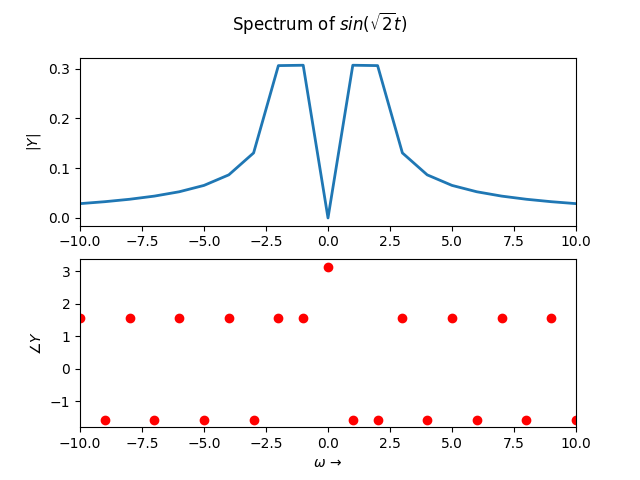
\includegraphics[scale=0.5]{Fig0.png}
        \caption{Spectrum of $sin(\sqrt{2}t)$}
        \label{fig:Fig0}
    \end{figure}
    
    But, this is not what we expected! We expected two peaks, but that is not what we got. This is because, we aren't finding out the DFT of the required function, $sin(\sqrt{2}t)$ :
    \begin{figure}
        \centering
        \includegraphics[scale=0.5]{fig10-2.png}
        \caption{$sin(\sqrt{2}t)$}
        \label{fig:fig10-2}
    \end{figure}
    
    \begin{figure}
        \centering
        \includegraphics[scale=0.5]{fig10-3.png}
        \caption{The function for which we are calculating DFT}
        \label{fig:fig10-3}
    \end{figure}
    
    We can see that this is not what we want to calculate the DFT for. The discontinuities in the function has led to the very problematic \textit{Gibb's Phenomenon}. So, we do not observe a sharp peak, but rather a flat one.
    
    This problem can be fixed by \textbf{windowing}. Windowing is an operation in which we multiply the time-domain function with a suitable window function. In this assignment, we choose the \textit{Hamming Window}, defined as:
    \begin{equation*}
        W_N[n] = \begin{cases}
                0.54 + 0.46\ cos(\frac{2\pi n}{N-1}),\  |n| < N\\
                0,\ otherwise
                \end{cases}
    \end{equation*}
    
    The result in time domain is that the magnitude of the jump is greatly reduced, thus minimizing the effect of Gibb's phenomenon in the frequency domain:
    \begin{figure}
        \centering
        \includegraphics[scale=0.5]{fig10-5.png}
        \caption{Windowed $sin(\sqrt{2}t)$}
        \label{fig:fig10-5}
    \end{figure}
    
    \begin{figure}
        \centering
        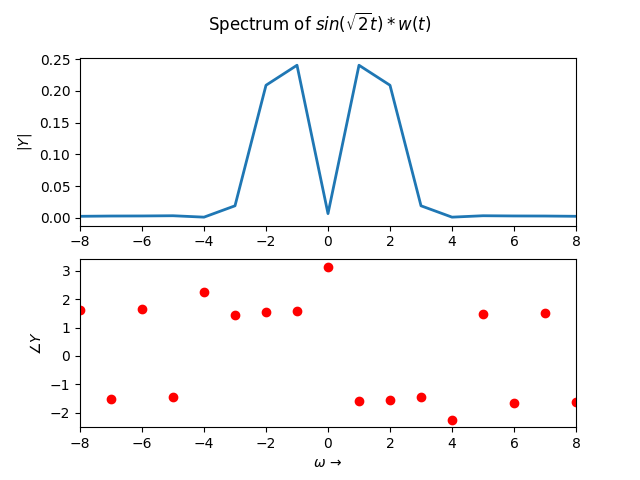
\includegraphics[scale=0.5]{Fig1.png}
        \caption{Spectrum of windowed $sin(\sqrt{2}t)$}
        \label{fig:Fig1}
    \end{figure}

\section{Spectrum of $cos^3(0.86 t)$}
    We can see the effect of windowing even better for $cos^3(0.86 t)$. We get the following spectra before and after windowing:
    \begin{figure}[H]
        \centering
        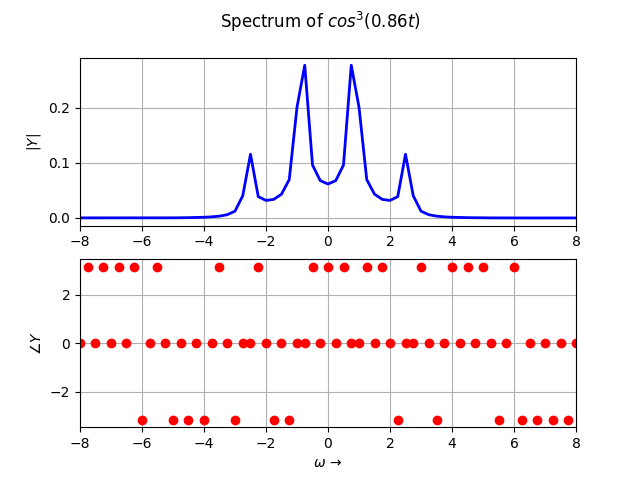
\includegraphics[scale=0.5]{Fig2.png}
        \caption{Spectrum of $cos^3(0.86 t)$ without windowing}
        \label{fig:Fig2}
    \end{figure}
    \begin{figure}[H]
        \centering
        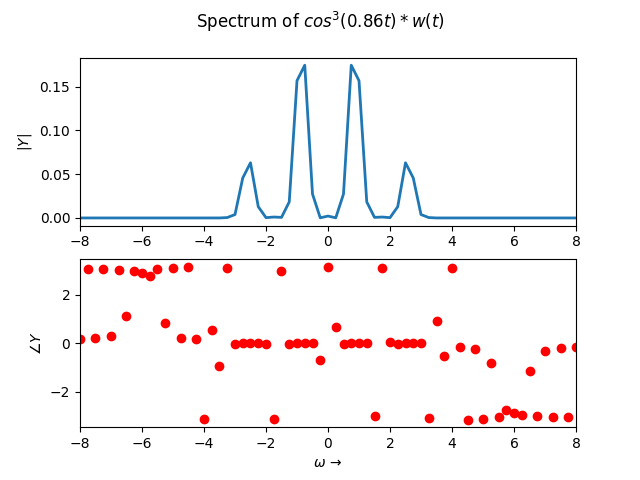
\includegraphics[scale=0.5]{Fig3.png}
        \caption{Spectrum of $cos^3(0.86 t)$ after windowing}
        \label{fig:Fig3}
    \end{figure}
    
    We can see narrower and sharper peaks at the frequencies that are present in the signal.

\section{Parameter Estimation using DFT}
    We are given a 128-element vector with sampled values of the signal $cos(\omega_ot+\delta)$, where $\omega_o$ and $\delta$ are to be estimated.
    
    We cannot extract $\omega_o$ from the DFT spectrum because the sampling rate is very low (only 128 points). The peaks will overlap and so we will not be able to extract their values.
    
    I used an approach as illustrated below:
    
    \begin{gather*}
        \omega_{o_{est}} = \frac{\sum_{\omega}|Y(j\omega)|^k\cdot \omega}{\sum_{\omega}|Y(j\omega)|^k}\\
        y(t) = Acos(\omega_ot) - Bsin(\omega_ot)\\
        \delta_{est} = \arctan(-\frac{B}{A})
    \end{gather*}
    
    In the above equations, I used a least squares approach to find A, B.
    
    I varied the parameter $k$ manually to find out which worked best for the given range of $\omega_o$. I used $k = 1.7$, for estimation in absence of noise, and $k = 2.4$, for estimation in presence of noise, to give the following results (I had set $\omega_o = 1.35$ and $\delta=\frac{\pi}{2}$ in both cases) :
    \vspace{3mm}
    \begin{table}[htbp]
        \centering
        \begin{tabular}{c|c|c|c|c}
            Noise & $\omega_o$ & $\omega_{o_{est}}$ & $\delta$ & $\delta_{est}$\\
            \hline
             0 & 1.35 & 1.453 & 1.571 & 1.571\\
             0.1*\texttt{rand($128$)} & 1.35 & 1.437 & 1.571 & 1.571\\
        \end{tabular}
        \label{tab:results}
    \end{table}
\section{DFT of chirp $cos(16t(1.5 + \frac{t}{2\pi}))$}
    A chirp is a signal in which the frequency increases or decreases with time\footnote{\textit{Source}: \href{https://en.wikipedia.org/wiki/Chirp}{https://en.wikipedia.org/wiki/Chirp}}. We are going to analyse the chirp signal $cos(16t(1.5 + \frac{t}{2\pi}))$. First, we shall plot the signal versus time, to get an idea of how the signal looks like:
    \begin{figure}
        \centering
        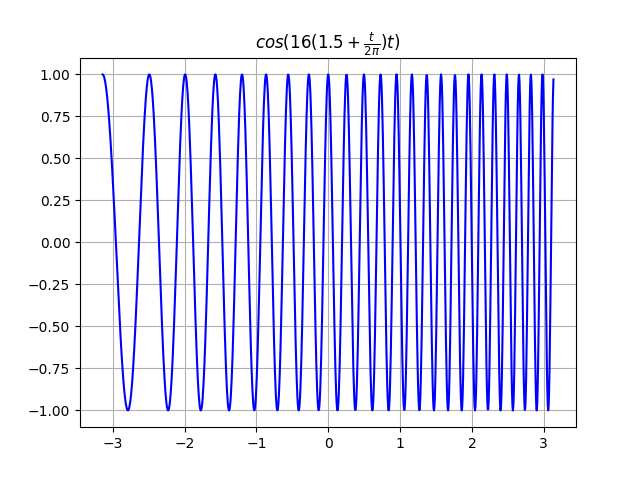
\includegraphics[scale=0.5]{Fig6.png}
        \caption{$cos(16t(1.5 + \frac{t}{2\pi}))$}
        \label{fig:Fig6}
    \end{figure}
    
    We see that the frequency varies from $16\ rad/sec$ to $32\ rad/sec$ as $t$ goes from $-\pi \ sec$ to $\pi\ sec$.
    
    On finding the DFT of the above signal, we get:
    \begin{figure}
        \centering
        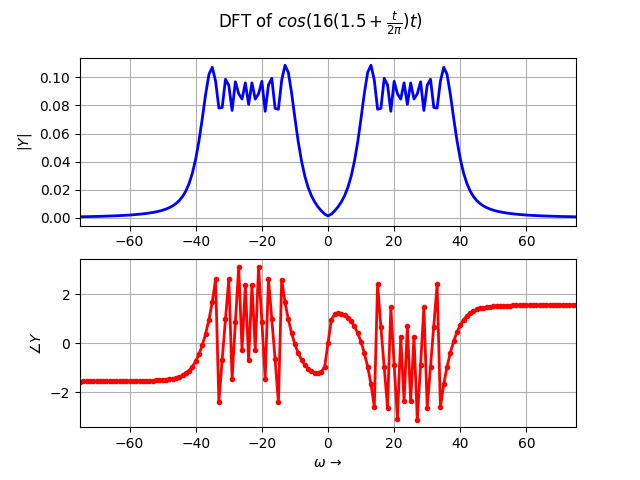
\includegraphics[scale=0.5]{Fig7.png}
        \caption{Spectrum of $cos(16t(1.5 + \frac{t}{2\pi}))$}
        \label{fig:Fig6}
    \end{figure}
    
    Applying the Hamming Window to the chirp results in the following:
    \begin{figure}[H]
        \centering
        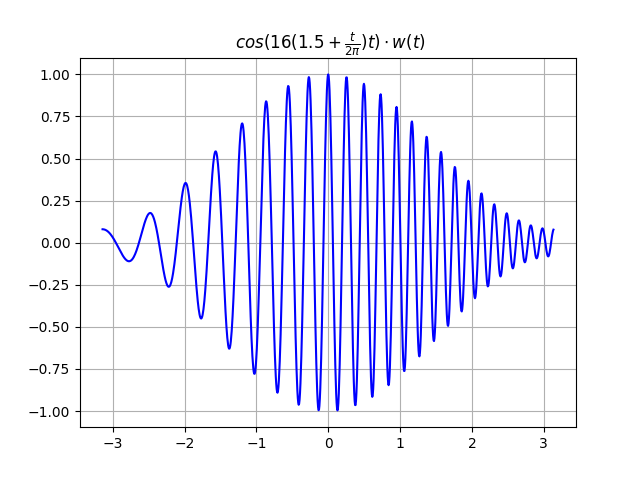
\includegraphics[scale=0.45]{Fig8.png}
        \caption{Windowed $cos(16t(1.5 + \frac{t}{2\pi}))$}
        \label{fig:Fig6}
    \end{figure}
    \begin{figure}[H]
        \centering
        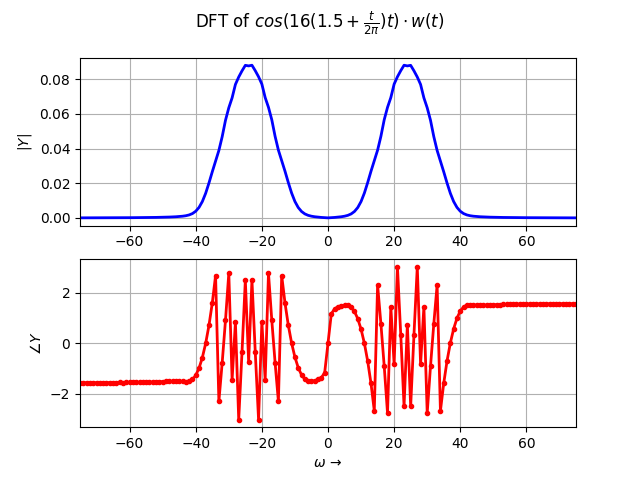
\includegraphics[scale=0.5]{Fig9.png}
        \caption{Spectrum of windowed $cos(16t(1.5 + \frac{t}{2\pi}))$}
        \label{fig:Fig6}
    \end{figure}
    
    The variations in the frequency have been smoothed out by the window, and also, we can see that the frequencies are more accurately confined to the range 16-32 $rad/sec$.

\section{Time-frequency plot of $cos(16t(1.5 + \frac{t}{2\pi}))$}
    We shall split the chirp in the time interval $[-\pi,\ \pi]$ into smaller intervals of time, and observe how the frequency of the signal varies with time.
    
    Initially we had a 1024-length vector with the values of the chirp signal. We shall split it into 64-length vectors, take the DFTs of these localized vectors, and plot a time-frequency surface plot to observe the variation of the frequency with time.
    
    \begin{figure}[H]
        \centering
        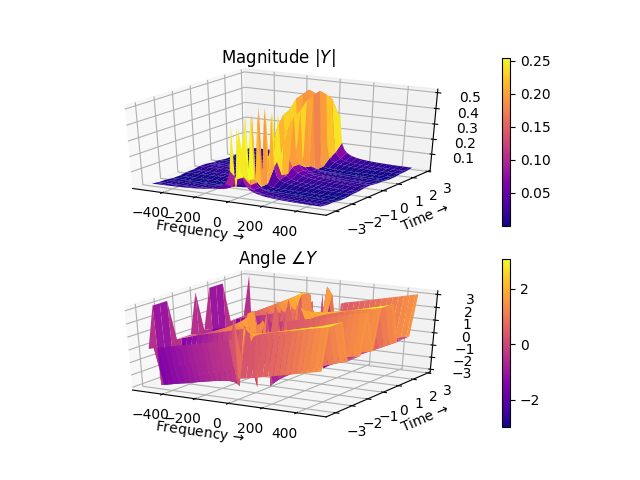
\includegraphics[scale=0.5]{Fig10.png}
        \caption{Spectrum of windowed $cos(16t(1.5 + \frac{t}{2\pi}))$}
        \label{fig:Fig6}
    \end{figure}
    \begin{figure}[H]
        \centering
        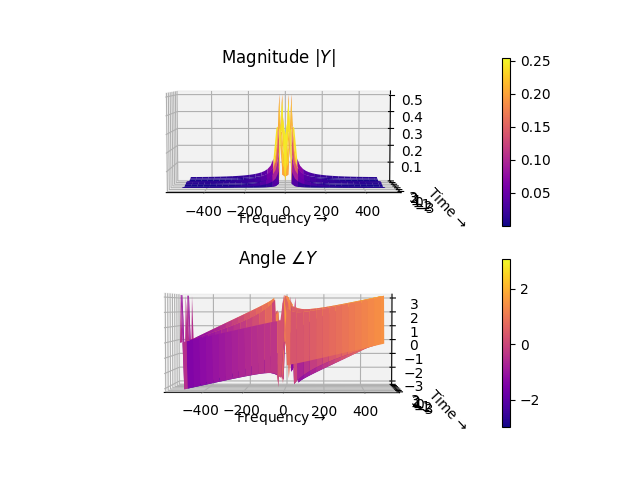
\includegraphics[scale=0.5]{Figure_10.png}
        \caption{Spectrum of windowed $cos(16t(1.5 + \frac{t}{2\pi}))$}
        \label{fig:Fig6}
    \end{figure}
    
    Now, we shall do the same, but with a windowed version of the chirp.
    \begin{figure}[H]
        \centering
        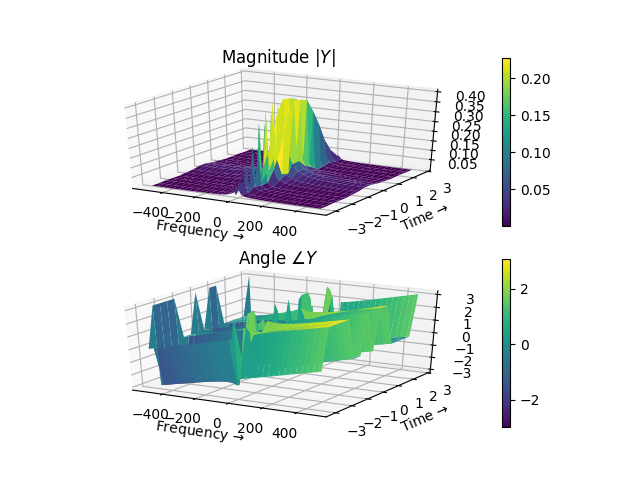
\includegraphics[scale=0.5]{Fig11.png}
        \caption{Spectrum of windowed $cos(16t(1.5 + \frac{t}{2\pi}))$}
        \label{fig:Fig6}
    \end{figure}
    \begin{figure}[H]
        \centering
        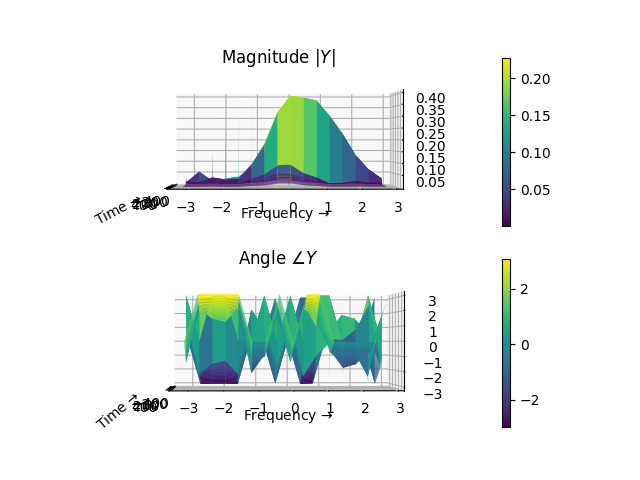
\includegraphics[scale=0.5]{Figure_11.png}
        \caption{Spectrum of windowed $cos(16t(1.5 + \frac{t}{2\pi}))$}
        \label{fig:Fig6}
    \end{figure}
    
    We can see that the change in the magnitude is more gradual in the windowed case.

\section{Conclusion}
    The DFT was obtained using a $2\pi$ periodic extension of the signal, and thus the spectrum was found to be erroneous for a non periodic function.  The spectrum was rectified by the using a windowing technique, by employing the Hamming window.  Given a vector of cosine values in the a time interval, the frequency and phase were estimated from the DFT spectrum, by using the expectation value of the frequency and a parameter tuning for optimum values.  The DFT of a chirped signal was analysed and its time-frequency plot showed the gradual variation of peak frequency of the spectrum with time.
\end{document}
